% Welcome! This is the unofficial University of Udine beamer template.

% See README.md for more informations about this template.

% This style has been developed following the "Manuale di Stile"
% (Style Manual) of the University of Udine. You can find the
% manual here: https://www.uniud.it/it/ateneo-uniud/ateneo-uniud/identita-visiva/manuali-immagine-stile/manuale-stile

% Note: for some reason, the RGB values specified in the manual
% do NOT render correctly in Beamer, so they have been redefined
% for this document using the high level chromo-optic deep neural 
% quantistic technology offered by Microsoft Paint's color picker.

% We defined four theme colors: UniBrown, UniBlue, UniGold
% and UniOrange. For example, to write some uniud-brownish
% text, just use: \textcolor{UniBrown}{Hello!}

% Note that [usenames,dvipsnames] is MANDATORY due to compatibility
% issues between tikz and xcolor packages.

\documentclass[10pt,usenames,pdf,hyperref={unicode},dvipsnames]{beamer}

% русский
%\usepackage[T2A]{fontenc}
\usepackage[english]{babel}
\usepackage[utf8]{inputenc}

\usepackage{amsmath}
\usepackage{amsfonts}
%\usepackage{bbm}

\usepackage{verbatim}
\usetheme{uniud}

% рисунки
\usepackage{graphicx, caption, subcaption}
\usepackage{tabularx}
\usepackage{multirow}
\usepackage{booktabs}
\usepackage{array}

%%% Bibliography
\usepackage[style=authoryear,backend=biber]{biblatex}
\addbibresource{biblio.bib}

% Author names in publication list are consistent 
% i.e. name1 surname1, name2 surname2
% See https://tex.stackexchange.com/questions/106914/biblatex-does-not-reverse-the-first-and-last-names-of-the-second-author
\DeclareNameAlias{author}{first-last}

%%% Suppress biblatex annoying warning
\usepackage{silence}
\WarningFilter{biblatex}{Patching footnotes failed}

%%% Some useful commands
% pdf-friendly newline in links
\newcommand{\pdfnewline}{\texorpdfstring{\newline}{ }} 
% Fill the vertical space in a slide (to put text at the bottom)
\newcommand{\framefill}{\vskip0pt plus 1filll}

\renewcommand{\footnotesize}{\scriptsize}

\title[]{{\large Моделирование спектров \\ столкновительно-индуцированного поглощения \\ в дальней ИК области \\ методом классических траекторий}}
\date[Июнь 2019]{4 июня, 2019}
\author[]{
  \vspace*{-1.0cm}
  \hfill \underline{Докладчик:} \\
  \hfill Финенко А. А. \\
  \vspace{0.5cm}
  \hfill \underline{Научные руководители:} \\
  \hfill с.н.с. к.ф.-м.н. Петров С.В. \\
  \hfill м.н.с. Локштанов С.Е. 
}
\institute{\vspace*{-1.9cm} \centering Химический факультет, МГУ им. М.В. Ломоносова \\ Кафедра физической химии \\ Лаборатория строения и квантовой механики молекул}

%\usepackage{xcolors}
\definecolor{darkolivegreen}{rgb}{0.33, 0.42, 0.18}
\definecolor{darkpastelgreen}{rgb}{0.01, 0.75, 0.24}

\newcommand{\hcancel}[1]{%
    \tikz[baseline=(tocancel.base)]{
        \node[inner sep=0pt,outer sep=0pt] (tocancel) {#1};
        \draw[red] (tocancel.south west) -- (tocancel.north east);
        \draw[red] (tocancel.south east) -- (tocancel.north west);
    }%
}%

\usepackage{physics}
\newcommand{\lb}{\left(}
\newcommand{\rb}{\right)}
\newcommand{\lsq}{\left[}
\newcommand{\rsq}{\right]}
\newcommand{\mean}[1]{\langle #1 \rangle}
\newcommand{\mf}{\mathbf}
\newcommand{\EOmega}{\boldsymbol{\Upsilon}_\mathbf{e}}
\newcommand{\bmu}{\boldsymbol{\mu}}

\newcommand{\intty}{\int\limits_{-\infty}^{+\infty}}

\newcommand{\mycaption}[2]{
    \textbf{#1:} #2
}

\newcommand{\bOmega}{\boldsymbol{\Omega}}
\newcommand{\Tl}{T_\text{L}}
\newcommand{\Th}{T_\text{H}}

\usepackage{csquotes}
\usepackage{dsfont}
\usepackage{bbm}

\newcommand{\bba}{\mathbbm{a}}
\newcommand{\bbA}{\mathds{A}}
\newcommand{\bbI}{\mathds{I}}
\newcommand{\bbG}{\mathds{G}}
\newcommand{\bbW}{\mathds{W}}

\begin{document}

\begin{frame}
\titlepage
\end{frame}

\begin{frame}{{\large Столкновительно-индуцированное поглощение (СИП)} \footfullcite{crawford1949}}
    \begin{block}{Вращательный переход запрещен в мономере}
        \vspace*{-0.5cm}
        \begin{gather}
            \hcancel{$N_2(j_A) + h \nu \rightarrow N_2(j_B)$} \notag
        \end{gather}
    \end{block}
    \begin{block}{Переход разрешен в столкновительном комплексе}
        \vspace*{-0.5cm}
        \begin{gather}
            \left\{ N_2 + N_2\right\}(J) + h \nu \rightarrow \left\{ N_2 + N_2 \right\}(J^\prime) \notag
        \end{gather}
    \end{block}
    \begin{block}{Состояния молекулярных пар}
        \begin{enumerate}
            \item \color{red}{Связанные состояния}
            \item \color{darkpastelgreen}{Континуальные свободные состояния} 
            \item \color{darkpastelgreen}{Метастабильные состояния} 
        \end{enumerate}
    \end{block}
\end{frame}

\begin{frame}{Приложения спектров СИП}
    \vspace*{-0.1cm}
    \begin{enumerate}
        \item N$_2-$N$_2$: атмосферы Земли и Титана \footfullcite{borysow1986} \\
        \item CO$_2-$Ar: атмосферы Марса и Венеры \footfullcite{fox1988} \\
    \end{enumerate}

    \begin{figure}[H]
        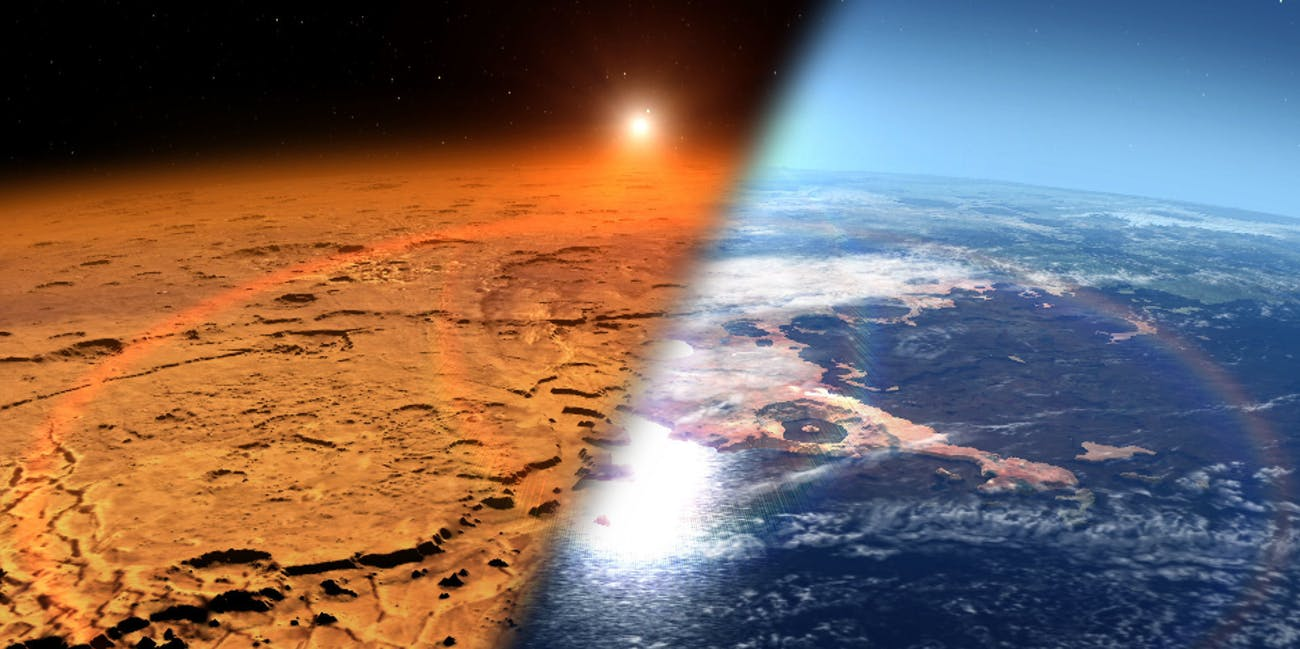
\includegraphics[width=0.49\linewidth, height = 3.9cm]{./pictures/early_mars.jpeg}
        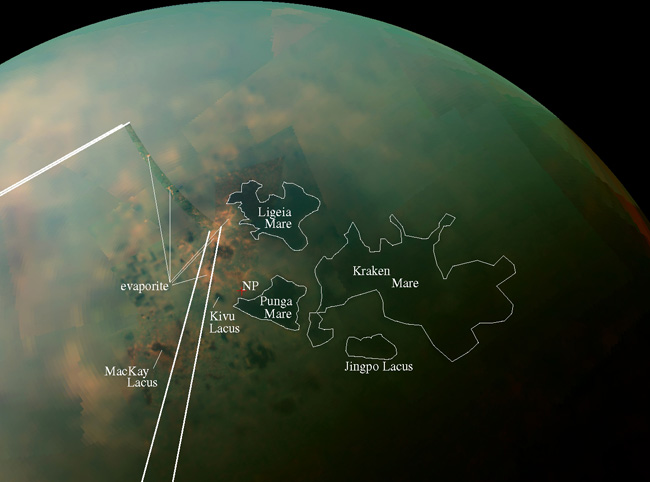
\includegraphics[width=0.49\linewidth, height = 3.9cm]{./pictures/titan.jpg}
        %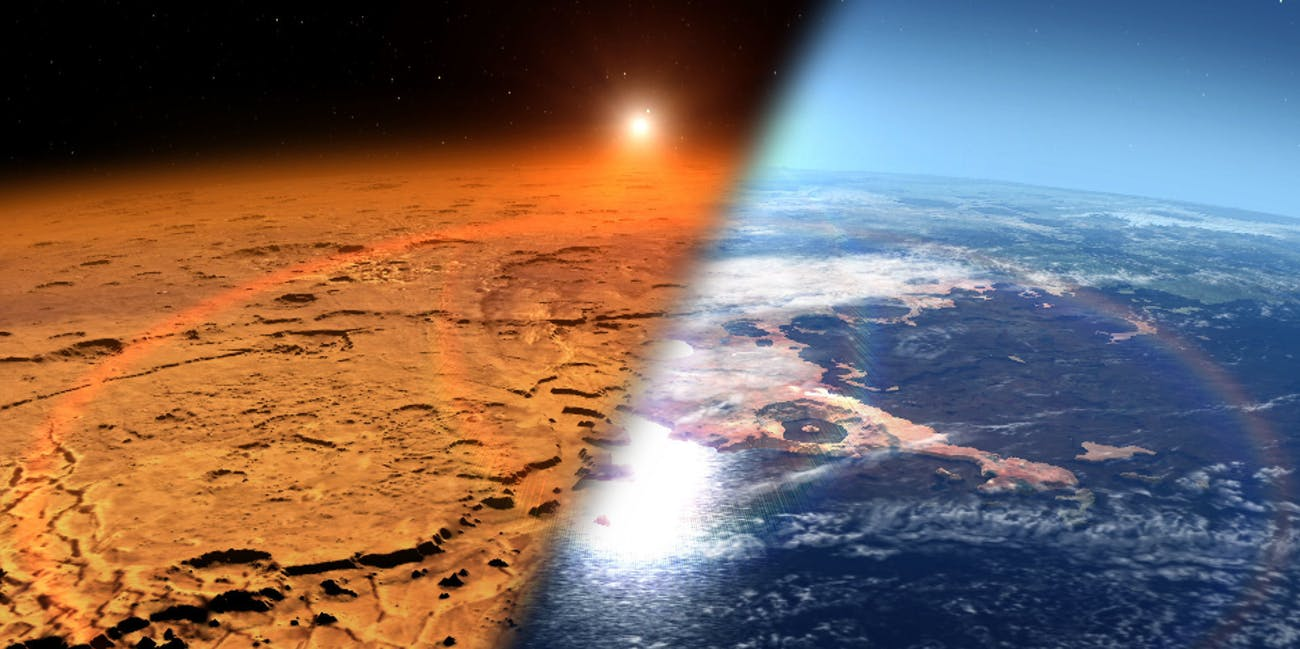
\includegraphics[width=5.0cm, height=3.8cm]{./pictures/early_mars.jpeg}
        %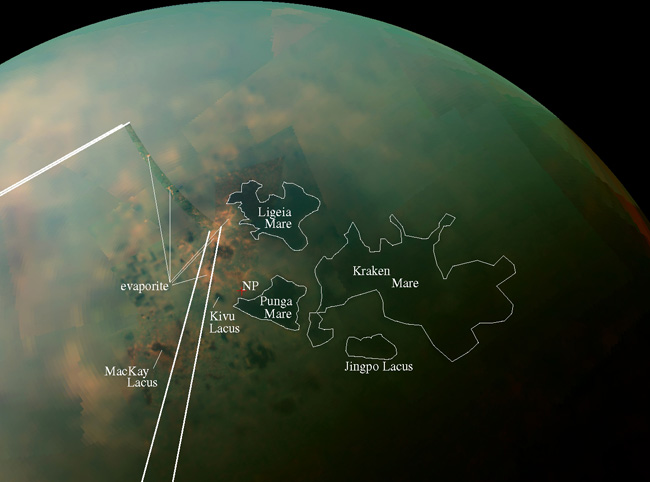
\includegraphics[width=5.0cm, height=3.8cm]{./pictures/titan.jpg}
        \mycaption{Рис. 1}{NASA/Cassini (справа)}
    \end{figure}
\end{frame}

\begin{frame}{{\large Взаимодействие молекул с электромагнитным полем}}
    \vspace*{-0.3cm}
    \begin{block}{Временная теория возмущений}
    \vspace*{-0.5cm}
	\begin{gather}
		i \hbar \frac{\partial \psi}{\partial t} = \hat{H} \psi, \quad \hat{H} = \hat{H}_0 + \lambda \hat{V}(t) \notag \\
        \lambda \hat{V}(t) = - \frac{E_0 (\bmu \cdot \boldsymbol{\varepsilon})}{2} \lb \exp \lb i \omega t \rb + \exp \lb - i \omega t \rb \rb \notag
	\end{gather}
\end{block}

\begin{block}{Коэффициент поглощения}
    \vspace*{-0.5cm}
	\begin{gather}
		\frac{\alpha(\nu)}{\rho_1 \rho_2} = \frac{(2 \pi)^3 N_L^2}{3 \hbar c} \nu \lsq 1 - \exp \lb - \frac{h c \nu}{k T} \rb \rsq V J(\nu) \notag \\ 
		J(\omega) = \sum_{\ket{i}, \ket{f}} \rho_i \Big{|} \bra{f} \hat{\boldsymbol{\mu}} \ket{i} \Big{|}^2 \delta \lb \omega_{fi} - \omega \rb \notag 
	\end{gather}
\end{block}
\end{frame}

\begin{frame}{{\large Спектральная функция и ее симметрия}}
    \vspace*{-0.8cm}
	\begin{gather}
		\begin{aligned}
            J_\text{квант.}(\omega) &= \frac{1}{2\pi} \int\limits_{-\infty}^{+\infty} dt \, e^{-i \omega t} \sum_i \rho_i \bra{i} \hat{\boldsymbol{\mu}}(0) \cdot \hat{\boldsymbol{\mu}}(t) \ket{i} \\ 
            J_\text{класс.}(\omega) &= \frac{1}{2\pi} \int\limits_{-\infty}^{+\infty} dt \, e^{-i \omega t} \mean{\bmu(0) \cdot \bmu(t)} \\ 
		\end{aligned} \notag
	\end{gather}

    \begin{figure}[H]
        \vspace*{-0.8cm}
        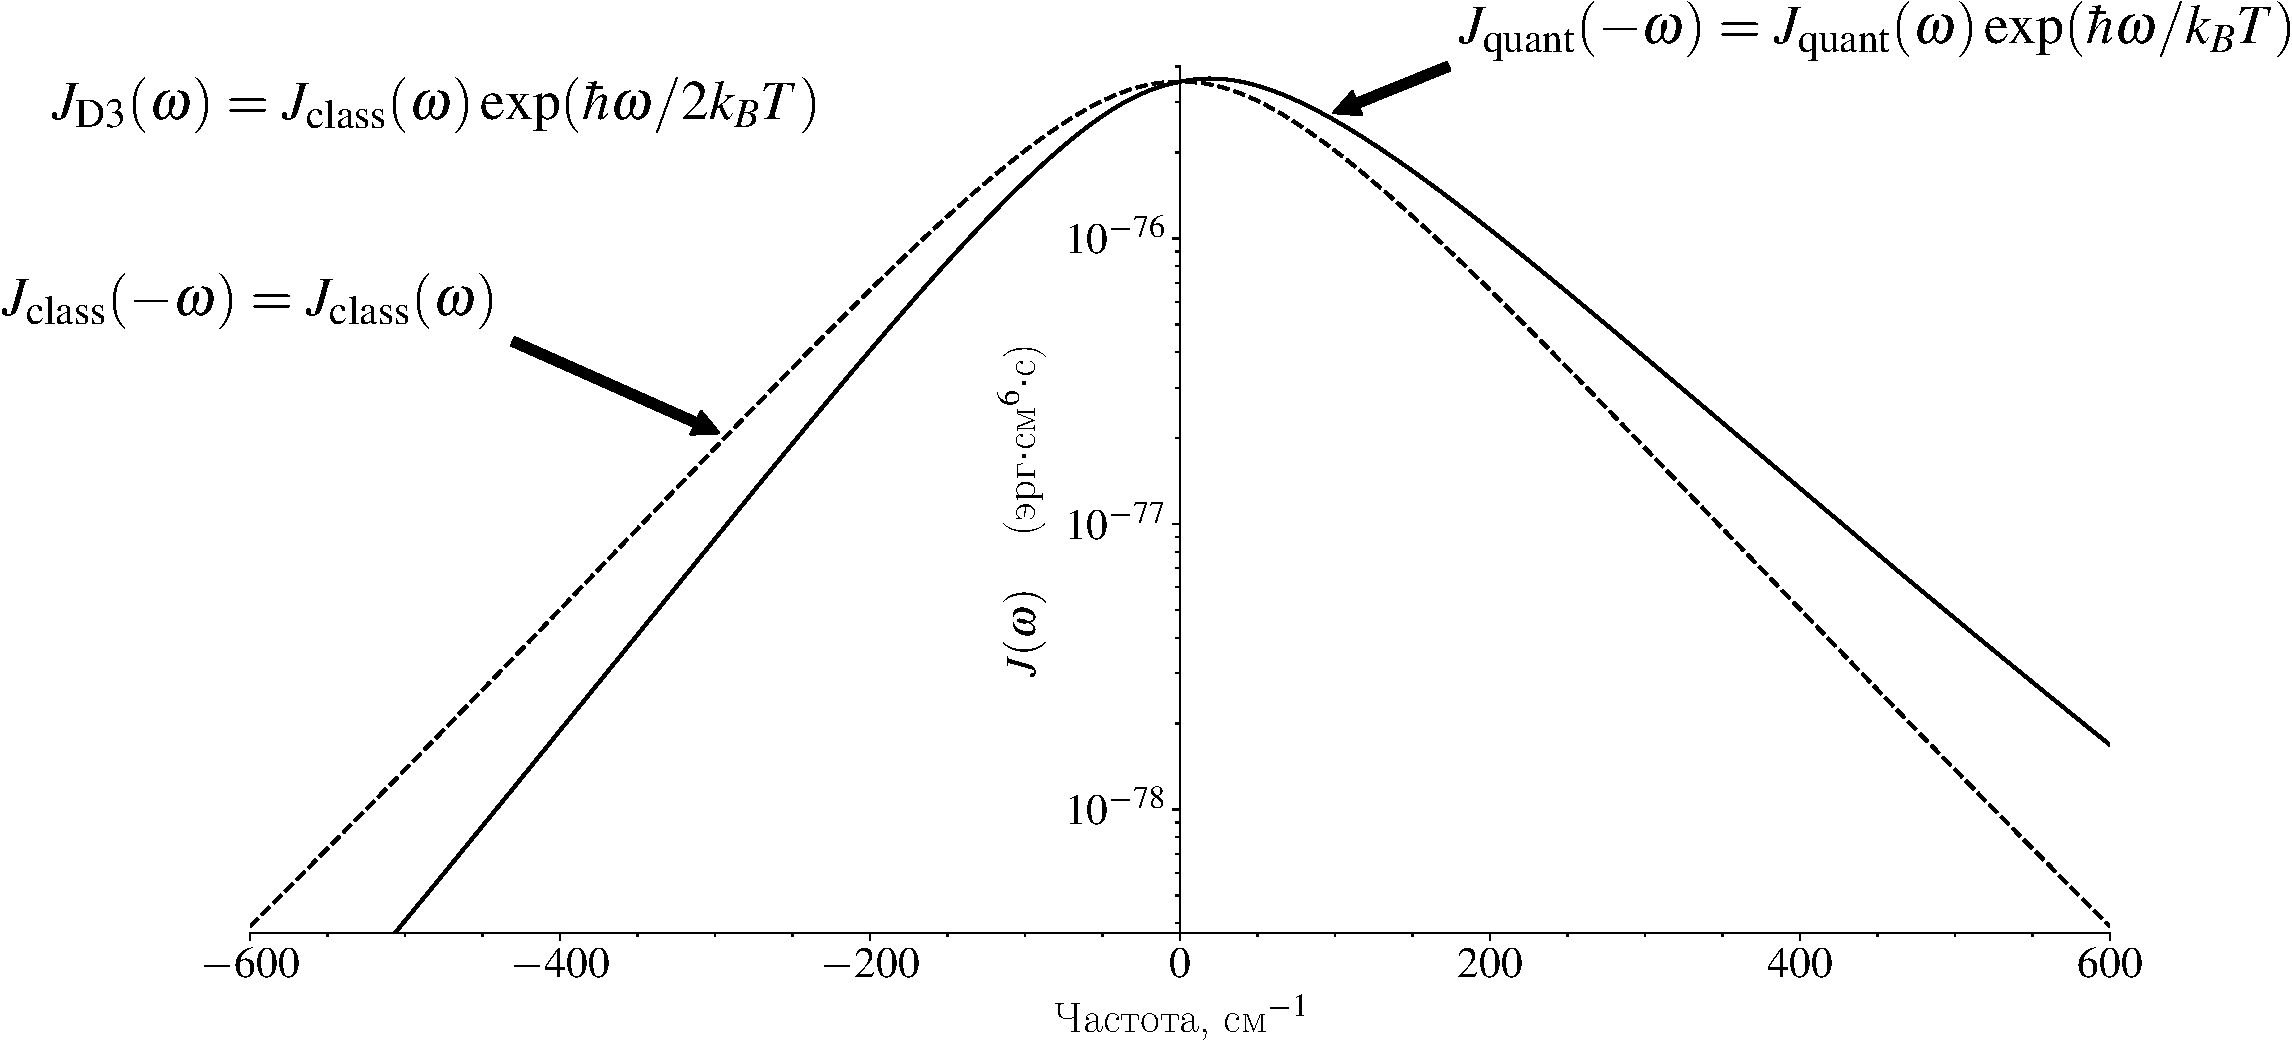
\includegraphics[width=\linewidth]{./pictures/spectral_function_symmetry-crop.pdf}
        %\caption{Картинка}
    \end{figure}

\end{frame}


\begin{frame}{Схема расчетной методики}
    \vspace*{-0.5cm}
    \begin{block}{Предварительная работа}
        \begin{enumerate}
            \item Введение обобщенных координат и вывод точного классического лагранжиана
            \item Аналитические аппроксимации \textit{ab initio} ППЭ и ПДМ
            \item Распределение начальных условий
        \end{enumerate}
    \end{block}
    \vspace*{-0.3cm}
    \begin{block}{Компоненты расчета методом классических траекторий}
        \begin{enumerate}
        \item Интегрирование уравнений движения для получения столкновительных траекторий
        \item Преобразование Фурье функции дипольного момента вдоль каждой стокновительной траектории
        \item Расчет классической спектральной функции усреднением по ансамблю траекторий рассеяния 
        \item Десимметризация спектральной функции и расчет бинарного коэффициента поглощения
        \end{enumerate}
    \end{block}
\end{frame}

\begin{frame}{Классический формализм}
    \vspace*{-0.5cm}
    \begin{figure}[H]
        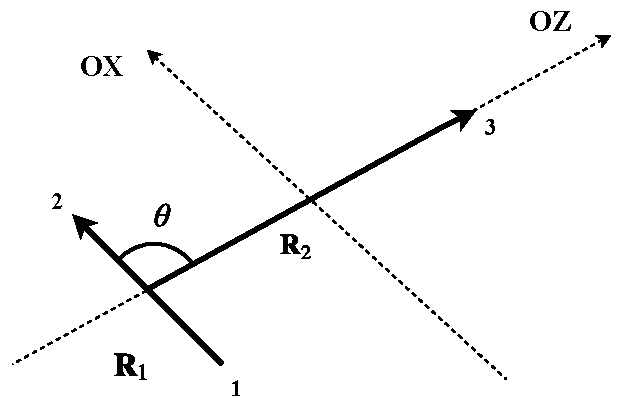
\includegraphics[width=0.49\linewidth]{./pictures/triatom_coordinates.pdf}
        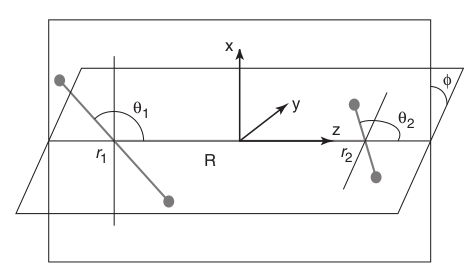
\includegraphics[width=0.49\linewidth]{./pictures/n2n2_coordinate_frame.png}
        \mycaption{Рис. 4}{Обобщенные координаты для систем атом$-$линейная молекула (слева) и линейная молекула$-$линейная молекула (справа)}
    \end{figure}
    \vspace*{-0.3cm}
    \begin{block}{Кинетическая энергия в форме Лагранжа и Гамильтона}
        \vspace*{-0.3cm}
        \begin{minipage}{0.6\linewidth}
            \begin{gather}
                \begin{aligned}
                    \Tl &= \frac{1}{2} \dot{\mf{q}}^+ \bba \dot{\mf{q}} + \bOmega^+ \bbA \dot{\mf{q}} + \frac{1}{2} \bOmega^+ \bbI \, \bOmega \\
                    \Th &= \frac{1}{2} \mf{J}^+ \bbG_{11} \mf{J} + \mf{J}^+ \bbG_{12} \mf{p} + \frac{1}{2} \mf{p}^+ \bbG_{22} \mf{p}
                \end{aligned} \notag
            \end{gather}
        \end{minipage}
        \begin{minipage}{0.39\linewidth}
            \begin{gather}
                \begin{aligned}
                    \bbG_{11} &= \lb \bbI - \bbA \bba^{-1} \bbA^{+} \rb^{-1} \\
                    \bbG_{12} &= -\bbG_{11} \bbA \bba^{-1} \\
                    \bbG_{22} &= \lb \bba - \bbA^{+} \bbI^{-1} \bbA \rb^{-1}
                \end{aligned} \notag
            \end{gather}
        \end{minipage}
    \end{block}
\end{frame}

\begin{frame}{Поверхности ППЭ и ПДМ}
    \begin{figure}[H]
        \vspace*{-0.5cm}
        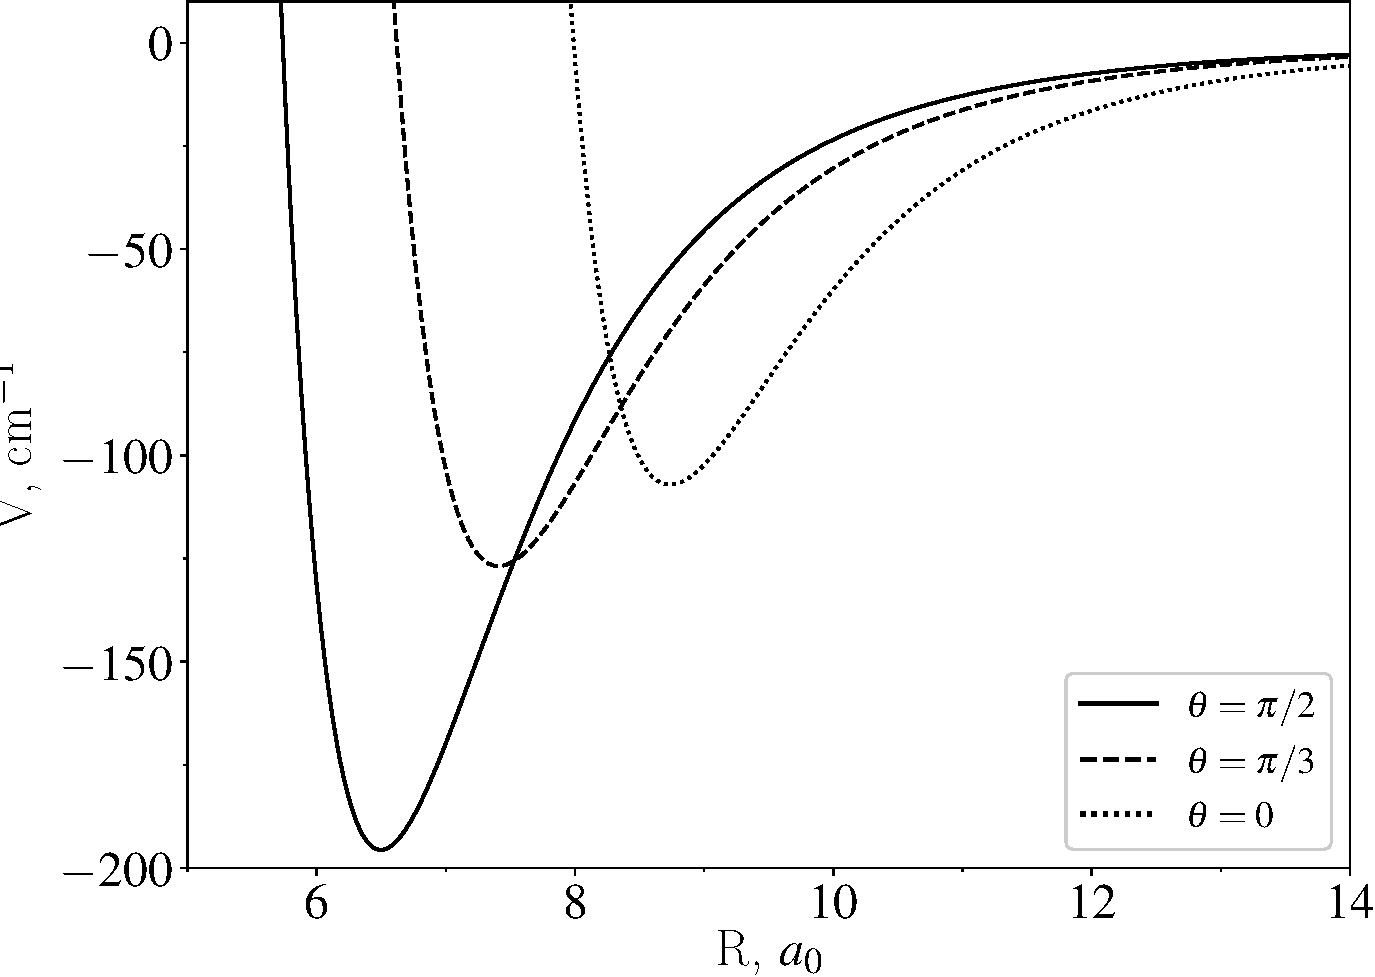
\includegraphics[width=0.49\linewidth]{./pictures/co2-ar-potential-legend-crop.pdf}
        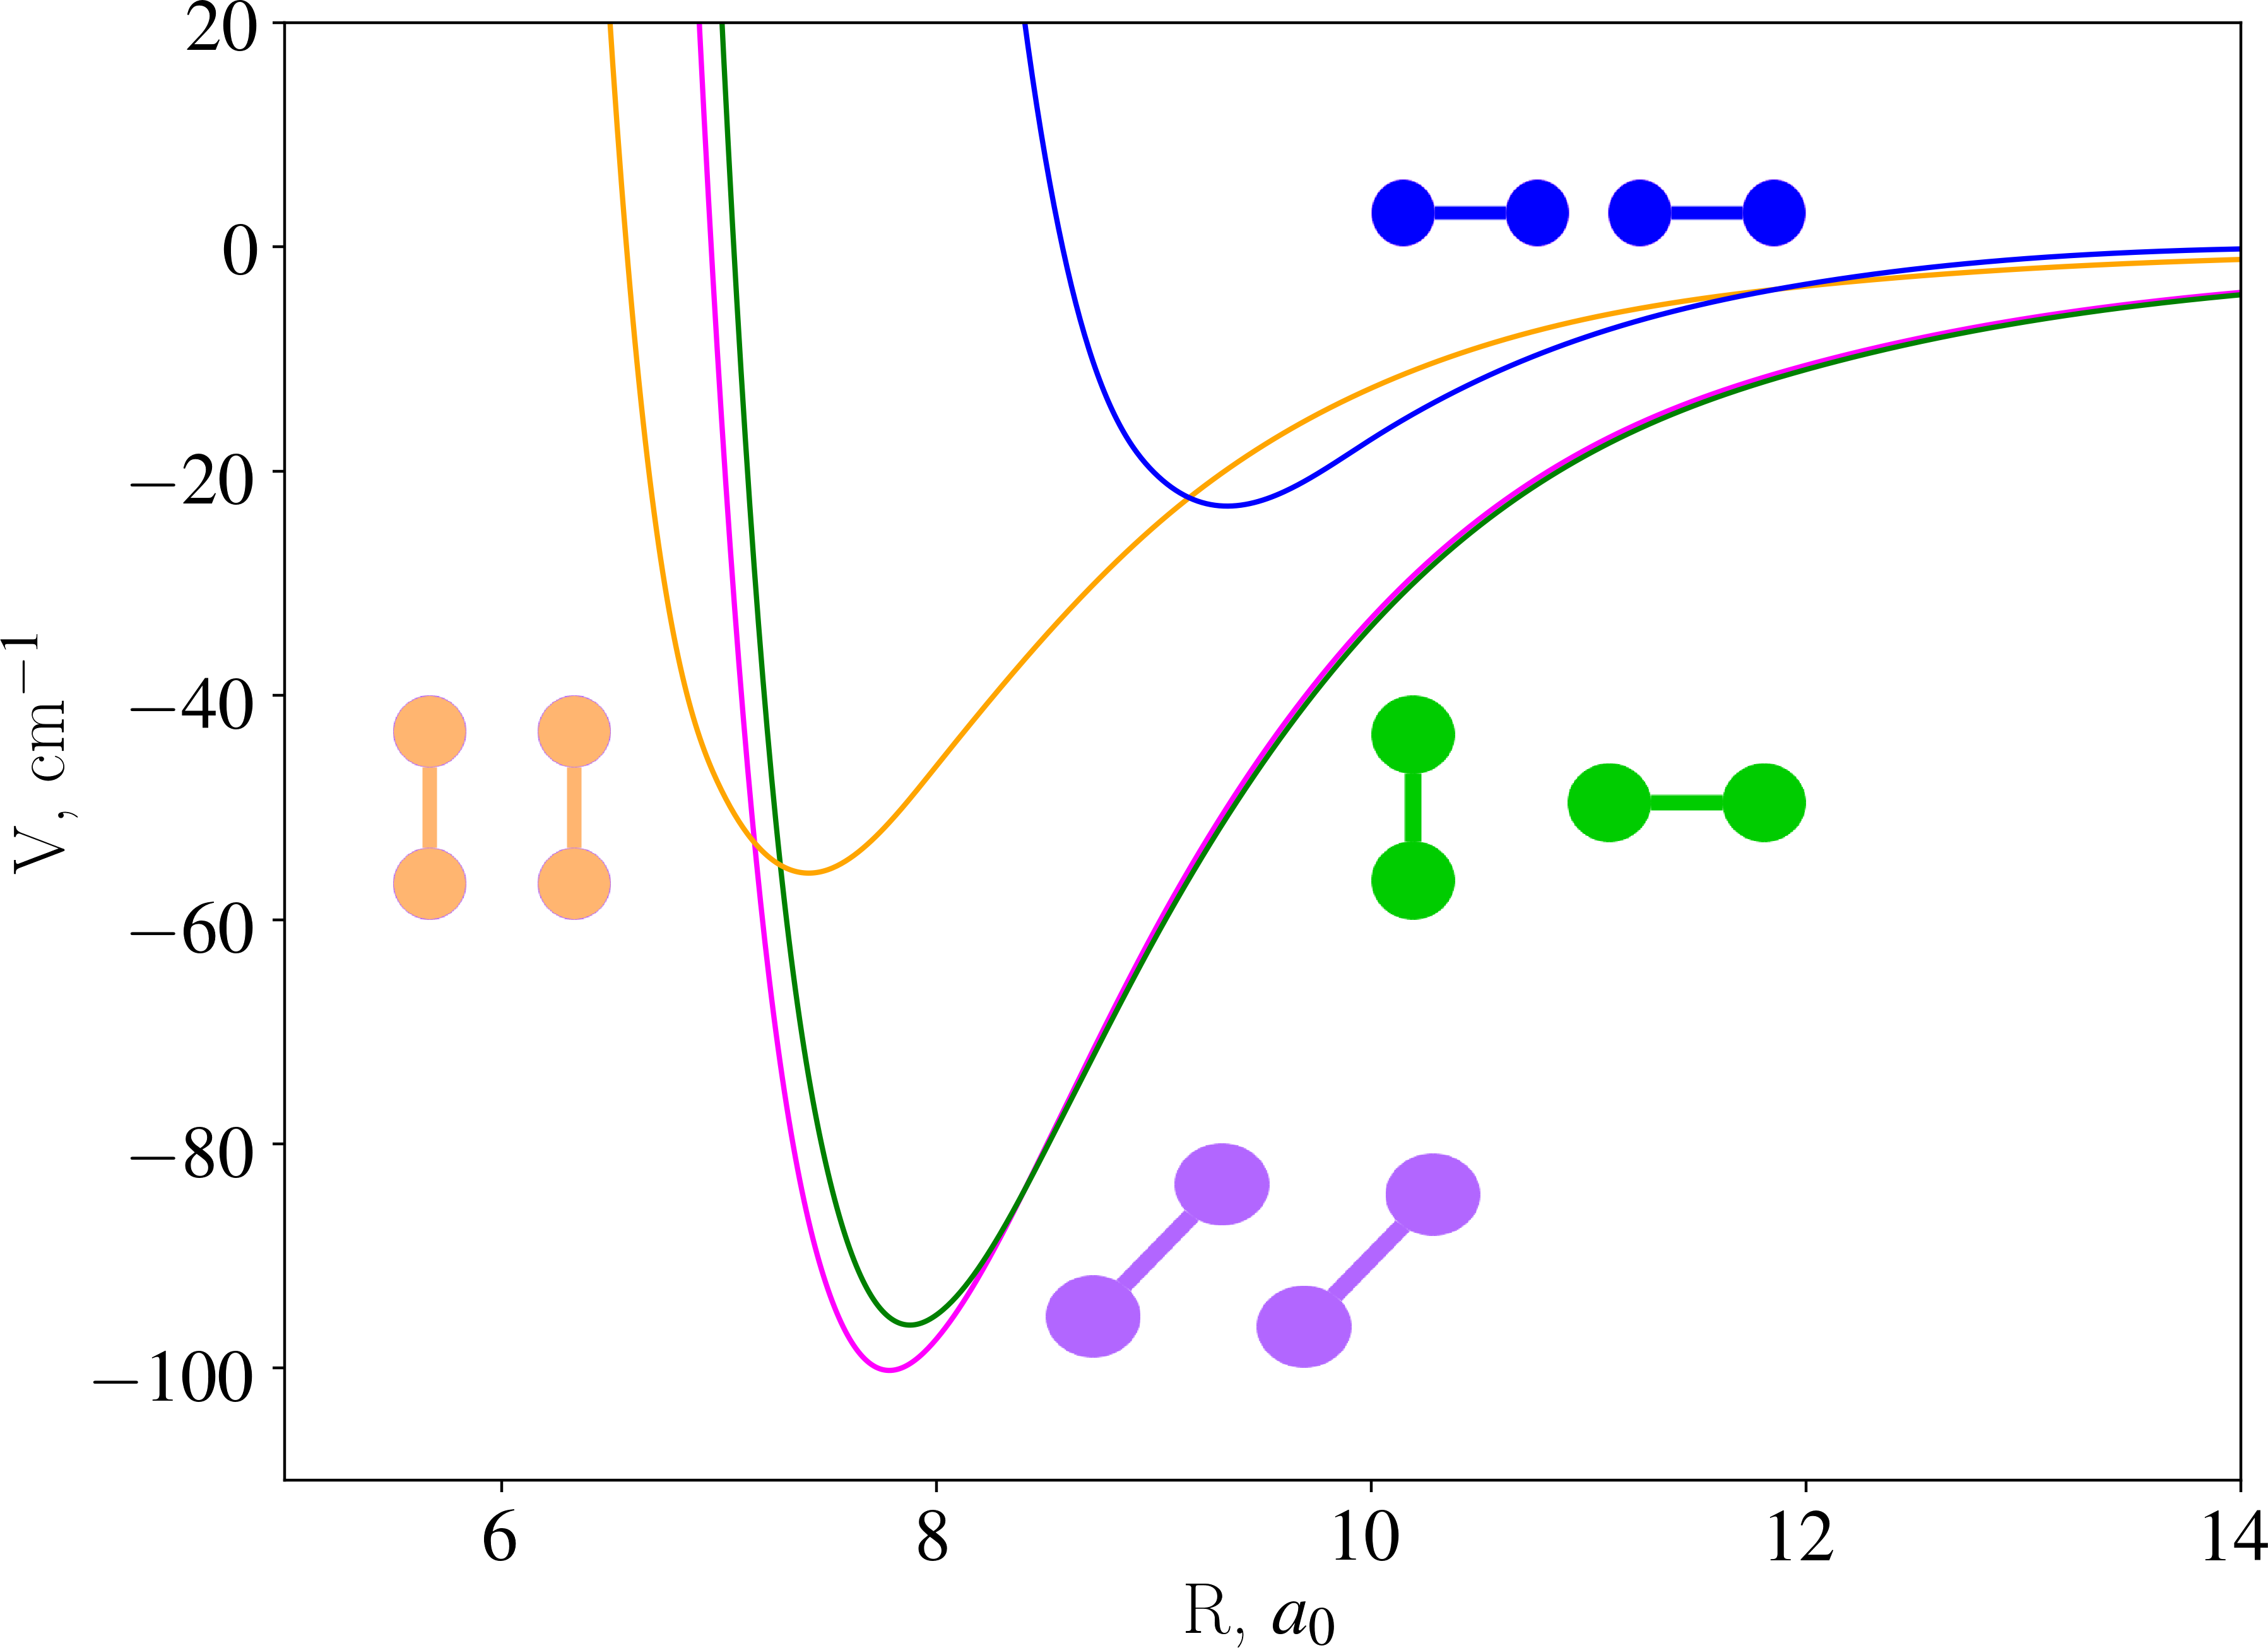
\includegraphics[width=0.49\linewidth]{./pictures/n2n2_potential-trim.png}
        \mycaption{Рис. 3}{Сечения ППЭ систем CO$_2-$Ar (слева) и N$_2-$N$_2$ (справа)}
    \end{figure}
   
    \vspace*{-0.3cm}
    \begin{itemize}
        \item ППЭ: CCSD(T)/\textit{aug}-cc-pVQZ, BSSE-коррекция
        \item ПДМ: Метод конечного поля, CCSD(T)/\textit{aug}-cc-pVTZ (CO$_2-$Ar), CCSD(T)/\textit{aug}-cc-pVQZ (N$_2-$N$_2$) \footfullcite{karman2015}, BSSE-коррекция
    \end{itemize}
\end{frame}

\begin{frame}{Метастабильные состояния}
    \vspace*{-0.5cm}
    \begin{figure}[H]
        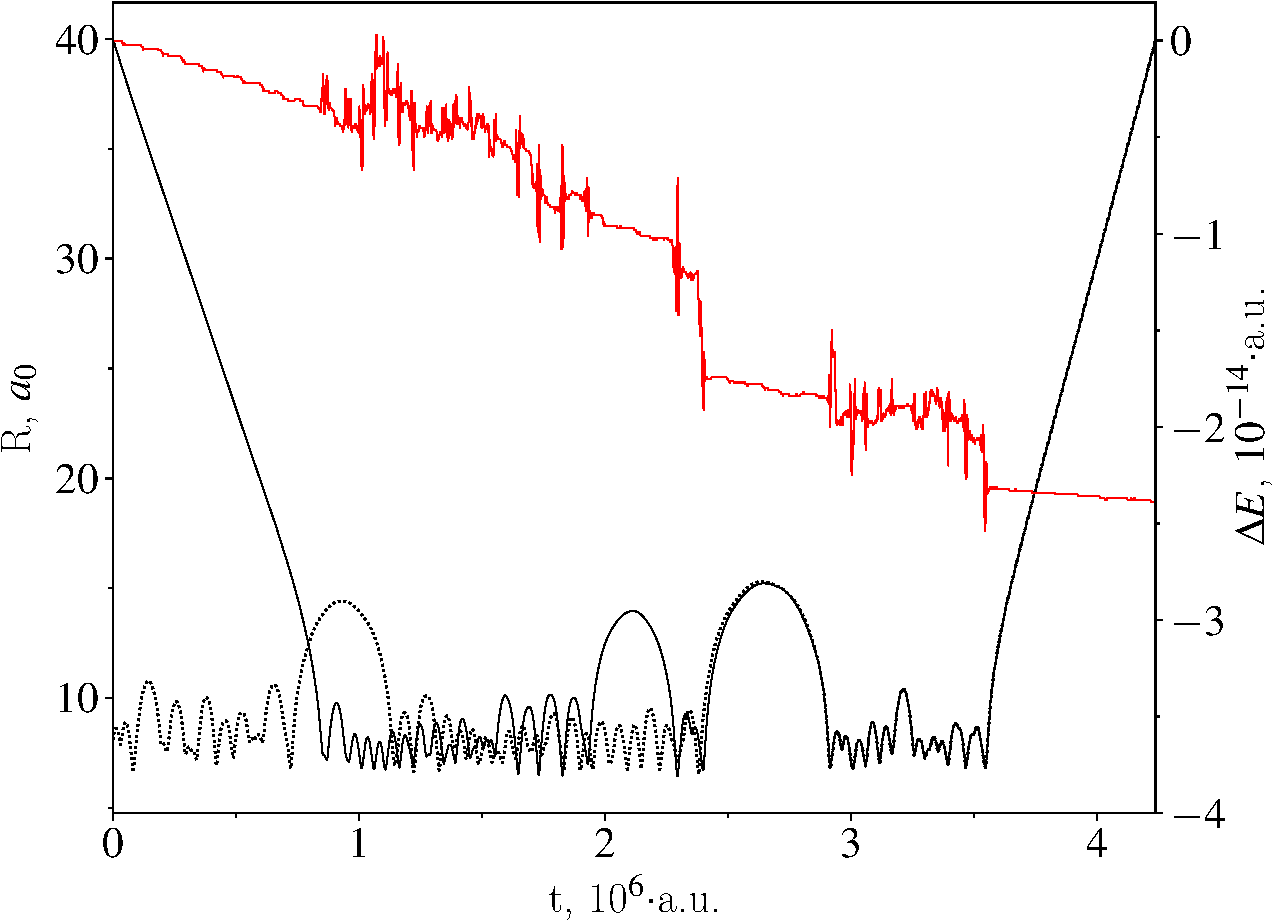
\includegraphics[width=0.8\linewidth]{./pictures/euler_trajectory-crop.pdf} \\
        \mycaption{Рис. 5}{Зависимости R(t) для прямой и обратной траекторий образования метастабильного комплекса N$_2-$N$_2$}
    \end{figure}
\end{frame}

\begin{frame}{Распределение начальных условий}
    \vspace*{-0.1cm}
	Метод Метрополиса-Хастингса для сэмплирования случайной величины с плотностью  
    \vspace*{-0.1cm}
    \begin{gather}
        \pi(\mf{q}, \mf{p}) = \frac{1}{\Gamma_0} \exp \lb -\frac{H(\mf{q}, \mf{p})}{k_B T} \rb \Bigg{|}_{r = r_\text{fixed}} \notag
    \end{gather}

    \vspace*{-0.5cm}
    \begin{figure}[H]
        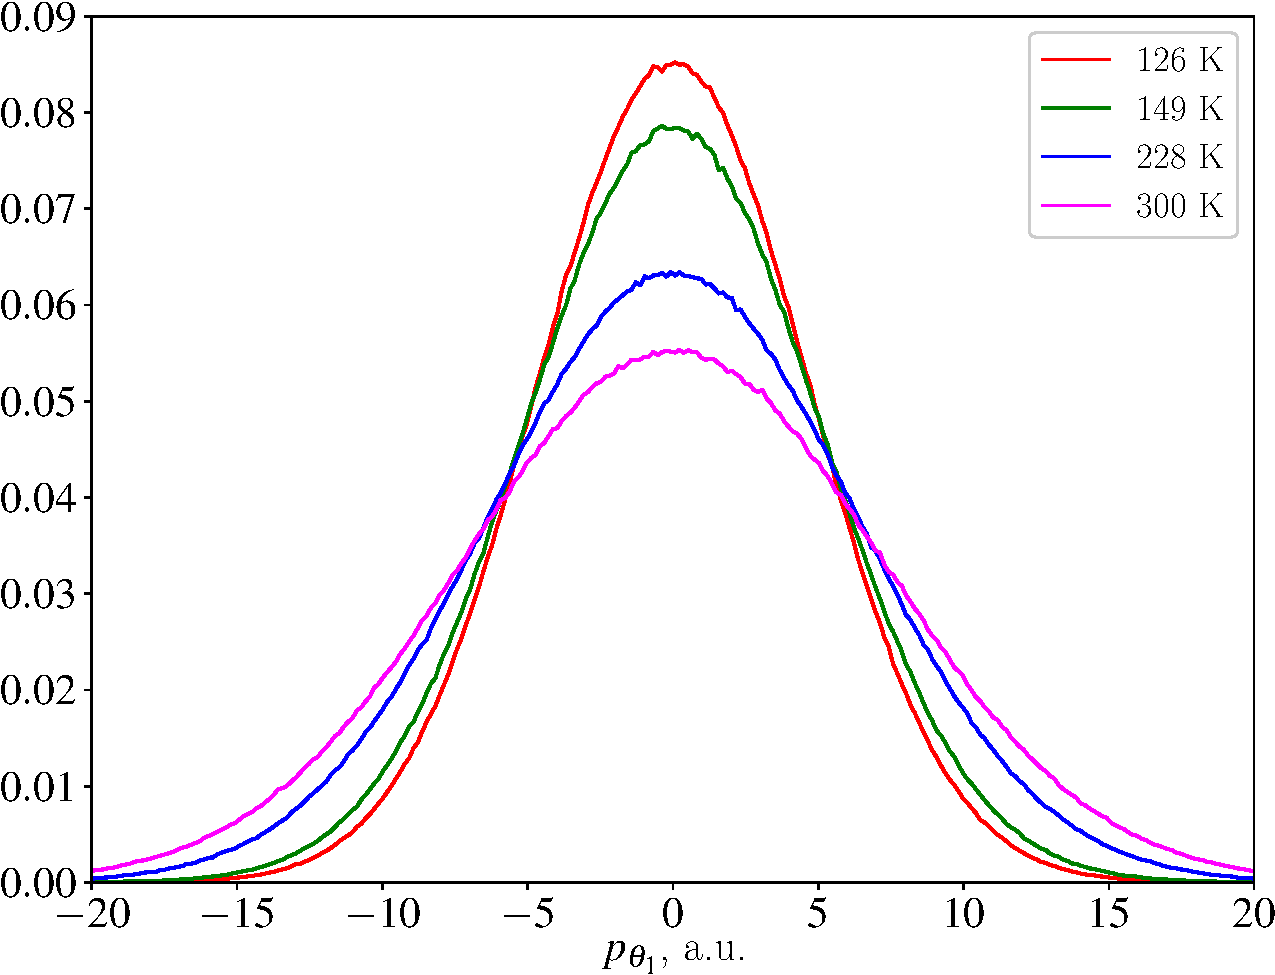
\includegraphics[width=0.49\linewidth]{./pictures/pTheta1-crop.pdf}
        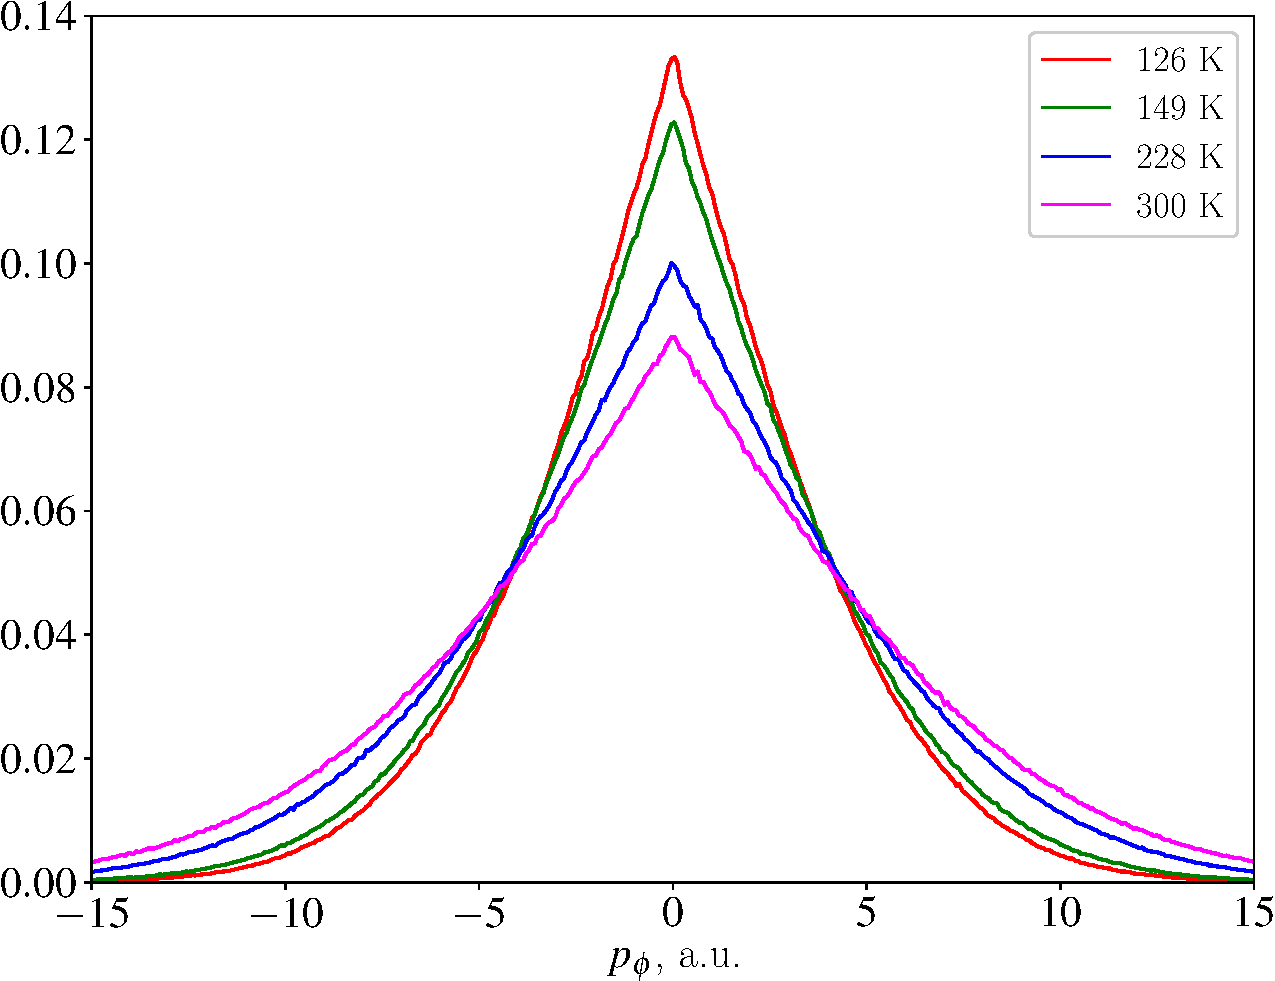
\includegraphics[width=0.49\linewidth]{./pictures/pPhi-crop.pdf}
        \mycaption{Рис. 6}{Распределения импульсов, сопряженных угловым координатам системы N$_2-$N$_2$}
    \end{figure}
\end{frame}

\begin{frame}{Приближения и неучитываемые эффекты}
    \begin{enumerate}
        \item \color{red}{Приближение Борна-Оппенгеймера} 
        \item Описание взаимодействия молекулярных систем с излучением в первом порядке ТВ
        \item Рассмотрение взаимодействия мономеров в рамках классической механики $\implies$ не учтены квантовые эффекты
        \item \color{blue}{Приближение \enquote{жестких мономеров}: неучет низших колебательных состояний}
        \item Волюнтаризм процедуры десимметризации
        \item \color{green}{Неучет связанных состояний}
    \end{enumerate}
\end{frame}

\begin{frame}{СИП N$_2-$N$_2$ в рототрансляционной полосе}
	\begin{center}
		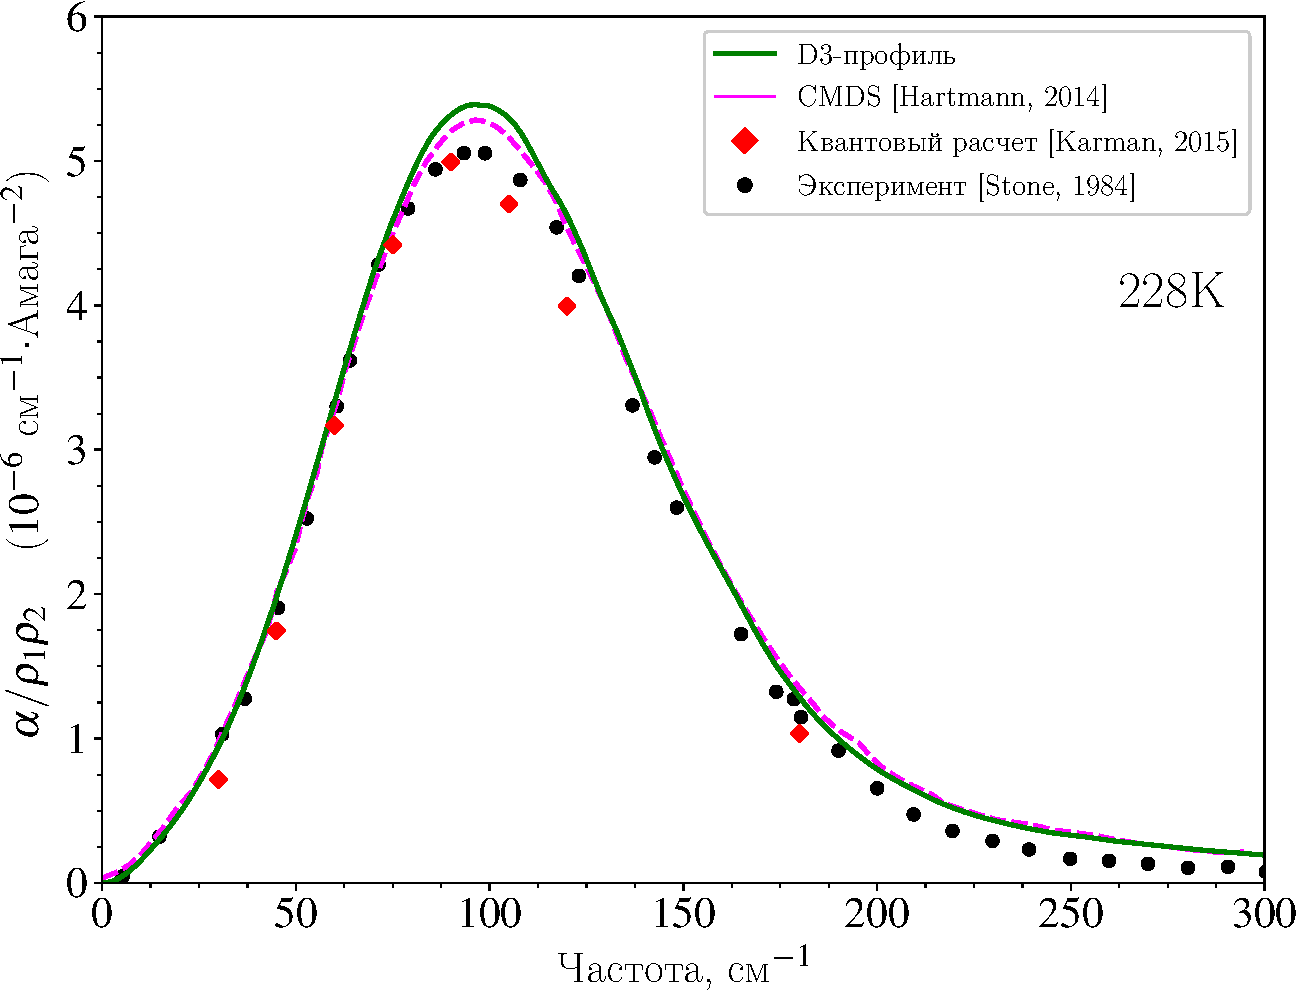
\includegraphics[width=0.9\textwidth]{./pictures/228K_russian_legend-crop.pdf}
	\end{center}
\end{frame}

\begin{frame}{СИП N$_2-$N$_2$ в рототрансляционной полосе}
	\begin{center}
		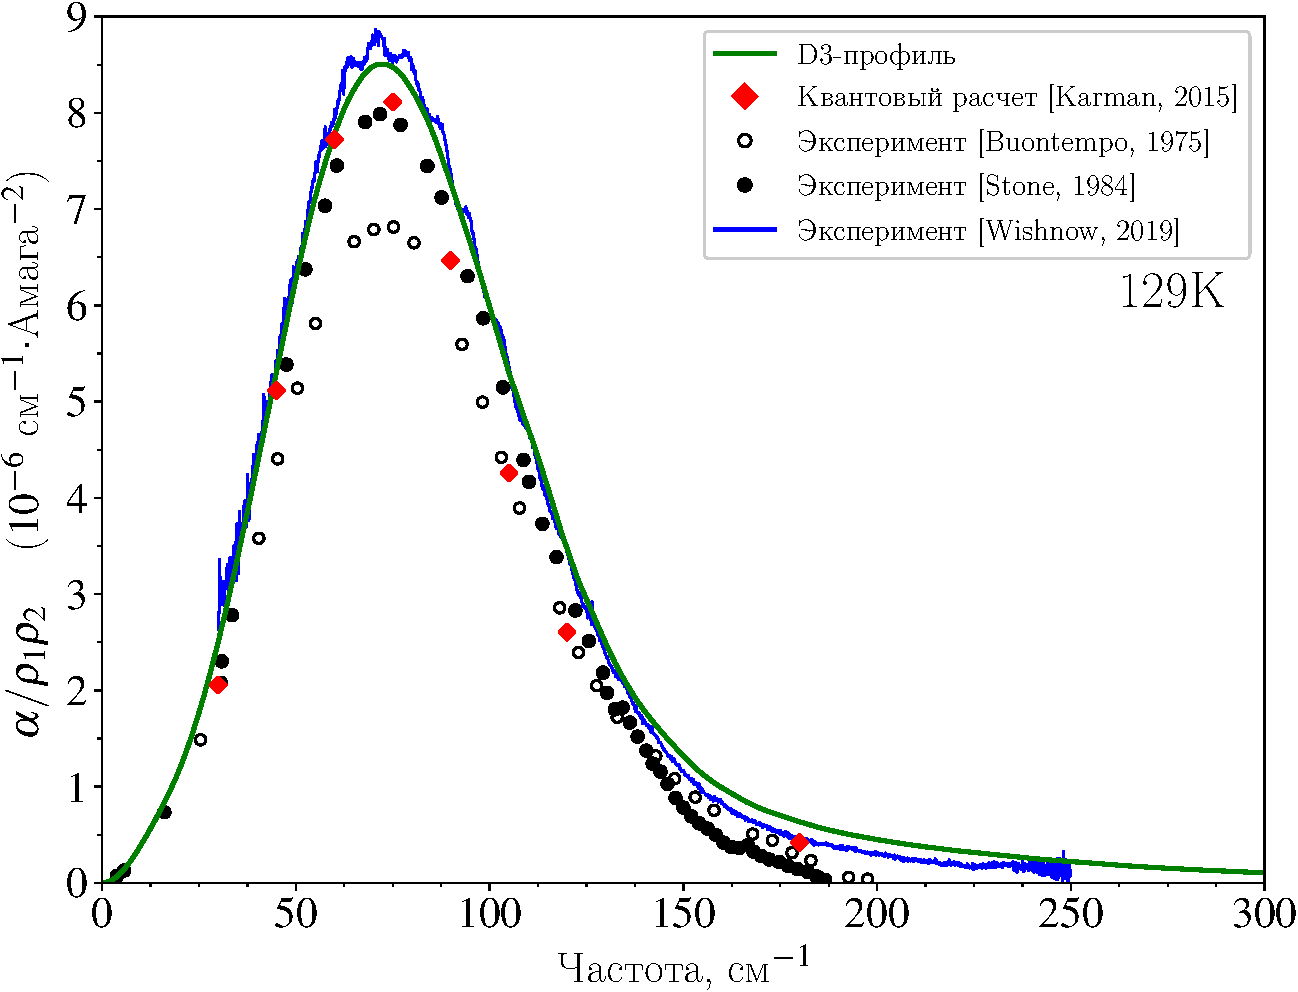
\includegraphics[width=0.9\textwidth]{./pictures/129K_russian_legend-crop.pdf}
	\end{center}
\end{frame}

\begin{frame}{СИП CO$_2-$Ar в рототрансляционной полосе}
	\begin{center}
		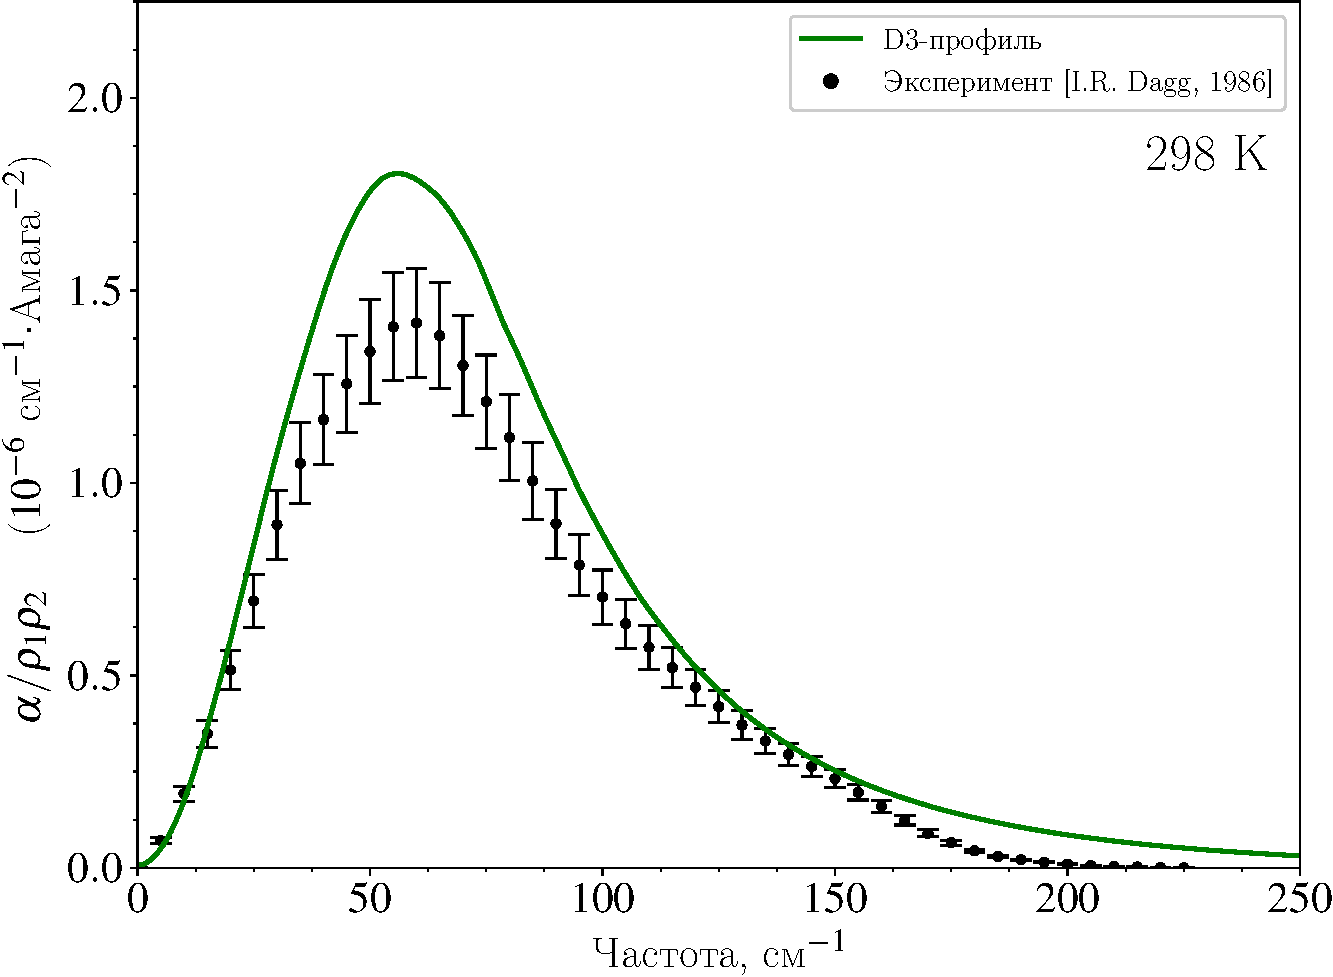
\includegraphics[width=0.9\textwidth]{./pictures/co2ar_298K-crop.pdf}
	\end{center}
\end{frame}

\begin{frame}{СИП CO$_2-$Ar в рототрансляционной полосе}
	\begin{center}
		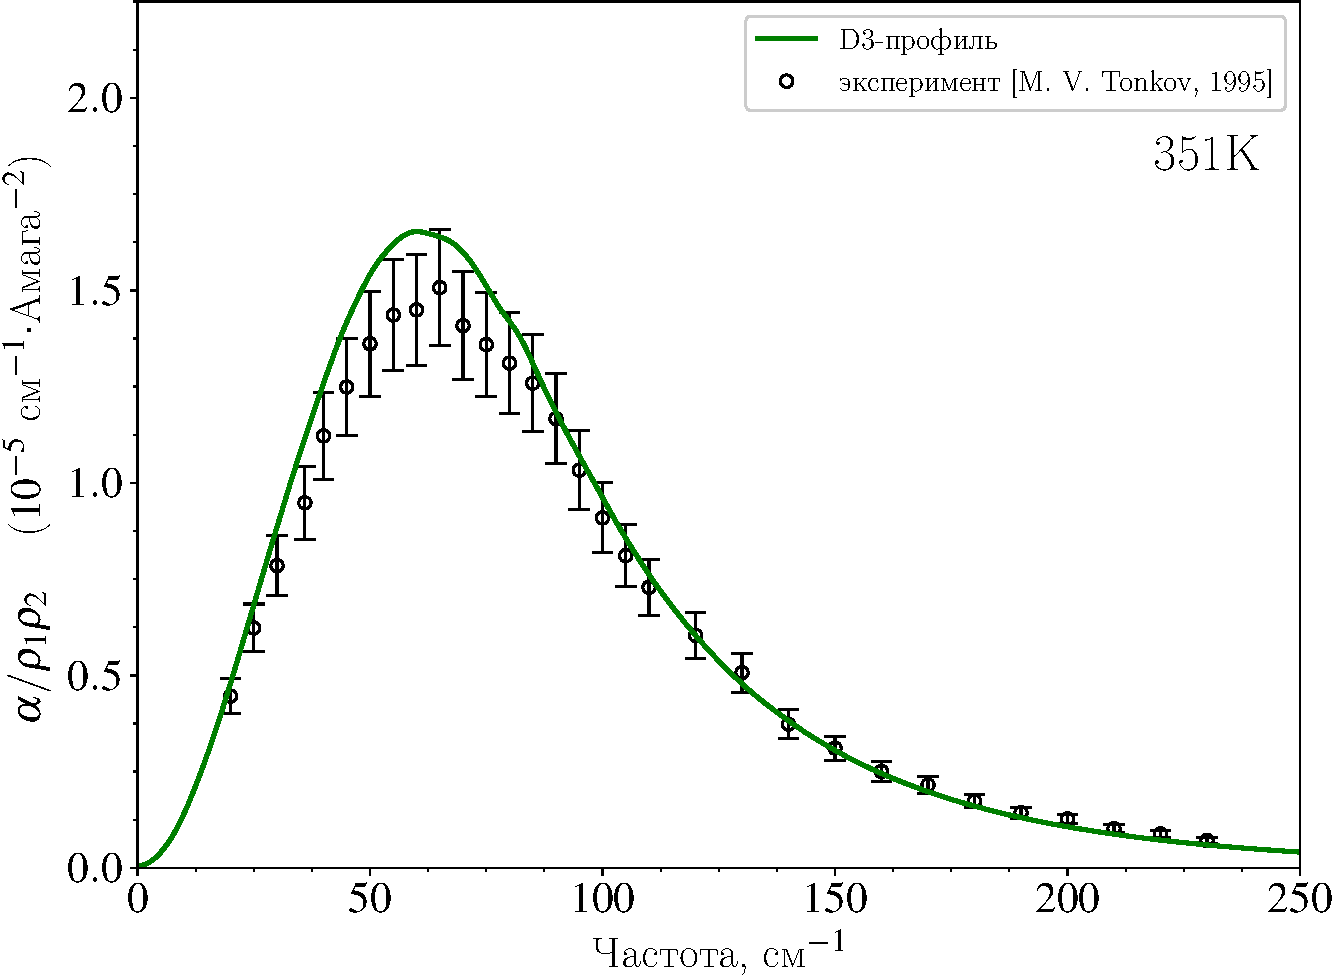
\includegraphics[width=0.9\textwidth]{./pictures/351K_russian_legend-crop.pdf}
	\end{center}
\end{frame}

\begin{frame}{\hspace*{-0.3cm}Спектральные моменты: контроль сходимости расчета}
    \vspace*{-0.3cm}
    \begin{block}{{\normalsize Интегралы по спектральной функции и по фазовому пространству}}
        \vspace*{-0.6cm}
        \begin{gather}
            M_n = \int\limits_{-\infty}^{+\infty} \nu^n VJ(\nu) d\nu \quad \Longleftrightarrow \quad 
            \begin{aligned}
                M_0 = \frac{\int \boldsymbol{\mu}^2 \exp \lsq -H \lb \mf{q}, \mf{p} \rb / k_B T \rsq d \mf{q} d\mf{p} }{\int \exp \lsq -H \lb \mf{q}, \mf{p}\rb / k_B T \rsq d \mf{q} d\mf{p} } \\
                M_2 = \frac{\int \boldsymbol{\dot{\mu}}^2 \exp \lsq -H \lb \mf{q}, \mf{p}\rb / k_B T \rsq d \mf{q} d\mf{p}}{\int \exp \lsq -H \lb \mf{q}, \mf{p} \rb / k_B T \rsq d \mf{q} d\mf{p} } 
            \end{aligned} \notag
        \end{gather}
    \end{block}

    \vspace*{-0.7cm}
    \begin{table}[H]
            \begin{tabular}{c >{\centering}p{5cm} >{\centering}p{2cm} >{\centering}p{2cm}}
            \toprule
            $T$, K & $M_0^\text{ФП}(H > 0) / M_2^\text{ФП} (H > 0)$  & $M_0^\text{траект.} / M_2^\text{траект.}$ & $\Delta$ \tabularnewline
            \midrule
            \multirow{2}{*}{$129.0$} & $4.444\cdot 10^{-5}$ & $4.414 \cdot 10^{-5}$ & $+0.7$ \%  \tabularnewline
                                     & $1.227\cdot 10^{-1}$ & $1.232 \cdot 10^{-1}$ & $-0.4$ \%  \tabularnewline
                                     \midrule
            \multirow{2}{*}{$228.3$} & $3.756\cdot 10^{-5}$ & $3.768 \cdot 10^{-5}$ & $+0.3$ \%  \tabularnewline
                                     & $1.848\cdot 10^{-1}$ & $1.859 \cdot 10^{-1}$ & $+0.6$ \%  \tabularnewline
                                     \midrule
        \end{tabular}
        \mycaption{Таблица 1}{Сравнение спектральных моментов, рассчитанных по фазовому пространству, с моментами по траекторным спектрам системы N$_2-$N$_2$}
        \label{table:n2n2-moments}
    \end{table}
\end{frame}

\begin{frame}{Выводы}
    \vspace*{-0.7cm}
    \begin{enumerate}
        \item {\scriptsize Развита методика расчета столкновительно-индуцированных спектров из первых принципов методом классических траекторий с применением обобщенных внутренних координат и подвижной системы осей. Ключевым элементом, обеспечивающим масштабируемость методики при рассмотрении многоатомных систем, является расчет производных гамильтониана \enquote{на лету} через матрицы лагранжиана и их производные}
        \item {\scriptsize Выполнен расчет столкновительно-индуцированных спектров систем N$_2-$N$_2$ и CO$_2-$Ar. Сравнение с экспериментальными данными, доступными при отдельных температурах, подтверждает работоспособность развиваемой расчетной методики и ее применимость для моделирования континуальных столкновительно-индуцированных спектров.}
        \item {\scriptsize Развиваемая методика позволяет рассчитывать спектры СИП для различных молекулярных пар в широком интервале температур. Рассчитанные спектры применимы в  ряде атмосферных и астрофизических приложений и могут быть включены в специализированный раздел спектроскопических баз данных, например, HITRAN-CIA. Определение границы применимости метода для получения надежных результатов требует дальнейшего анализа и накопления расчетных данных для б\'{о}льшего числа молекулярных пар.} 
    \end{enumerate}
\end{frame}

\begin{frame}{}
    \centering
    {\Huge Спасибо за внимание!}
\end{frame}

\begin{frame}{Замена переменных с внедрением времени}
    \vspace*{-1.2cm}
    \begin{gather}
        \hspace*{-0.3cm}
        J(\omega) = \frac{1}{2 \pi} \hat{F} \Big[ \langle \bmu(0) \bmu(t) \rangle \Big] \rightarrow \frac{1}{2 \pi \Gamma_0} \int\limits_0^\infty \frac{p_r}{\mu} dp_r \int \exp \lb -\frac{H}{k_B T} \rb \Bigg\vert \hat{F} \Big[ \bmu(t) \Big] \Bigg\vert^2 d\boldsymbol{\Gamma}^\prime \notag
    \end{gather}
    \vspace*{-0.8cm}
    \begin{figure}[H]
        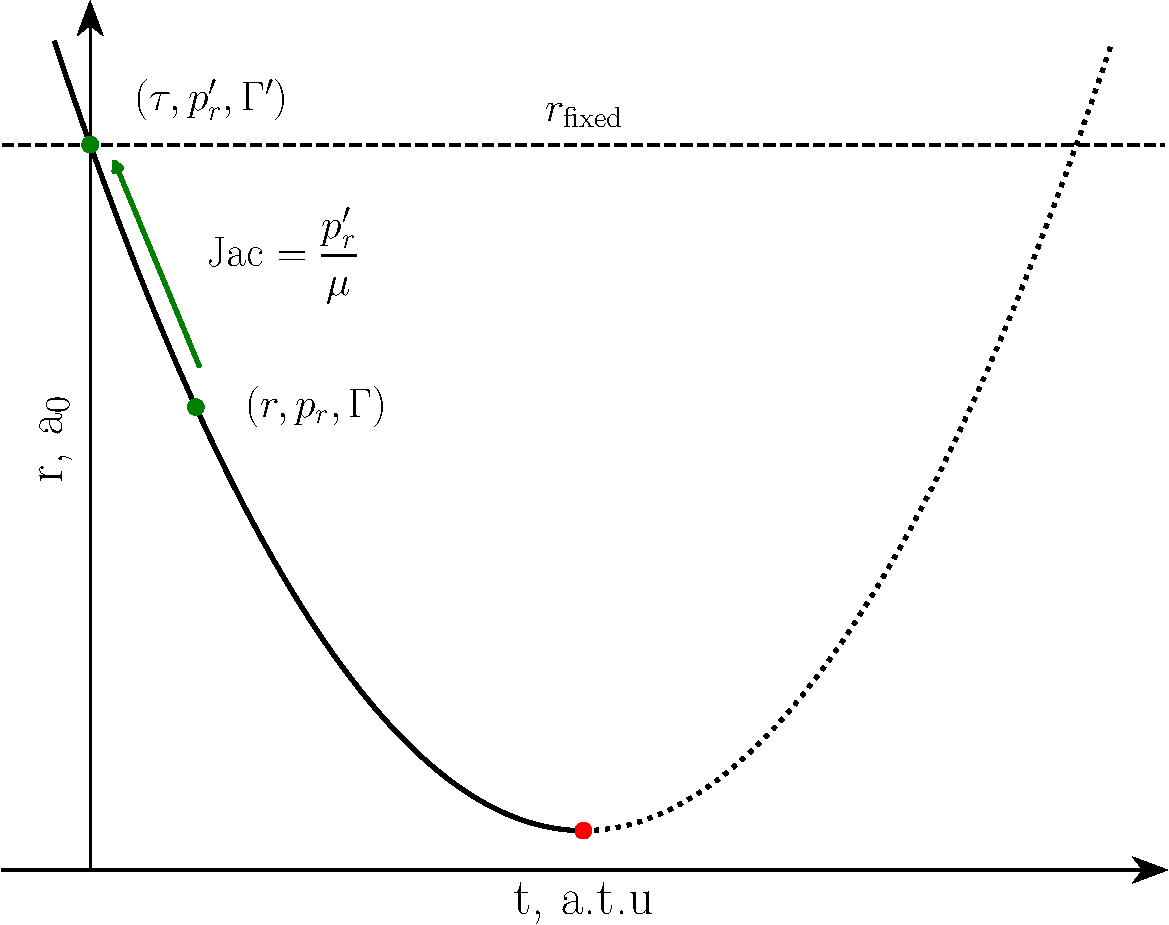
\includegraphics[width=0.75\linewidth]{./pictures/time-change-crop.pdf}
    \end{figure}
\end{frame}

\end{document}



